
\chapter*{Introduction}
\addstarredchapter{Introduction}

\chapter{État de l'art sur la détection de communautés et les réseaux dynamiques}
\minitoc
\label{chap:etat_art}
Dans cette thèse, nous étudions deux axes de recherches liés aux graphes qui sont orthogonaux.
D'une part, il s'agit de la détection de structures dans les graphes et plus particulièrement de communautés.
Un communauté est un sous-ensemble de n\oe uds de manière à ce qu'ils soient fortement connectés.
Il n'existe cependant aucune définition exact et la notion de communauté fortement connectée dépends du contexte et de la méthode.
Malgré cette définition floue, des structures communautaires ont été trouvées dans de nombreux graphes dans plusieurs domaines tel que le réseaux constitué des région du cerveau \cite{DeReus2014}, le réseau de distribution d'eau \cite{DiNardo2015} et un réseau d'interactions d'animaux \cite{Farine2015}.
Ces notions de communautés et les méthodes de détection sont définies dans la section~\ref{sec:intro_communaute}.\\

D'autre part, il a été observé que la modélisation d'un réseau sous la forme d'un graphe peut poser problème notamment quand le réseau change au cours du temps \cite{Holme2015b}.
D'une part, l'information temporelle est complètement perdue lorsque l'on manipule un graphe.
Par conséquent, certaines structures peuvent devenir indétectable.
Imaginons un graphe représentant les alliances politiques dans un pays.
Si toutes les alliances politiques sont agrégées sur une trop grande durée temporelle, alors une personne politique changeant de parti politique sera faussement considérée comme influente car connectée à plusieurs partis alors qu'elle peut ne plus avoir de contact dans son ancien parti.
Ainsi il n'est plus possible d'observer le glissement des alliances politiques dans ce genre de réseau si l'agrégation temporelle est trop importante~\cite{Mucha2010}.

D'autre part, si on prends en compte le temps, alors il est possible de détecter des structure plus fine que dans le cas statique.
Il devient possible de détecter des instant où l'organisation générale change~\cite{Rosvall2010}, de comprendre à quels sont les instant où une personnes est importante~\cite{Magnien2015}, ou bien de détecter des groupes temporelles~\cite{Cazabet2010}.
Face à ces problèmes plusieurs extensions de la théorie des graphes ont été proposées et elles sont résumées dans la section~\ref{sec:intro_extension_temporelle}.

Mais avant de présenter ces deux axes de recherches, nous revenons dans la section~\ref{[sec:def_graphe]} sur quelques définitions formelles et notation des graphes que nous utilisons dans cette thèse.
\section{Définition dans les graphes}
\label{sec:def_graphe}

Un graphe $G$ est défini par un couple $(V, E)$  où $V$ est une ensemble de n\oe uds et $E$ un ensemble de liens chaque lien est une paire de n\oe uds.
Sauf mention contraire, nous considérons des graphes non-orienté, c'est-à-dire pour toute pair de n\oe uds $u,v \in V$ les liens $(u,v)$ et $(v,u)$ sont équivalents.
Nous considérons également uniquement des liens non-pondérés, c'est-à-dire qu'un lien est soit présent soit absent.
Enfin, nous ne considérons que des graphes simples, c'est-à-dire qu'il n'existe au maximum qu'un seul lien entre deux n\oe uds.
Ceci est en opposition avec les graphes multiples où il peut exister plusieurs liens entre deux n\oe uds.

Par convention, nous définissons $n=|V|$ le nombre de n\oe uds et $m=|E|$ le nombre de liens.
Il est possible de représenter un graphe $G$ par une matrice carré $A$ de taille $n$ où la case $A_{i,j} \ \forall i,j \in \mathbb{N}^+ \leq n$ est égale à $1$ si un lien relie les n\oe uds $i$ et $j$ et $0$ sinon.


Le degré d'un n\oe ud $i$, noté $d_i$, est égale au nombre de liens reliés à $i$: $d_u = \sum_{j\leq n} A_{i,j}$.

Une chaine ou chemin entre deux n\oe uds dans un graphe est une suite de liens $((u_1,v_1),...,(u_k,v_k))$ de tel sorte que $v_{i}=u_{i+1} \ \forall i \in [0,k-1]$.
Les n\oe uds d'un graphe sont dit connexe s'il existe un chemin entre toute les pairs de n\oe uds.
Une composante connexe est un ensemble de n\oe uds $V'\subseteq V$ qui est connexe et maximal, c'est-à-dire qu'il n'est pas possible d'ajouter un n\oe ud dans $V'$ tel que $V'$ soit toujours connexe.

La densité, $d(G)$ dans un graphe est la probabilité que deux n\oe uds soient reliés par un lien: $d(G)=\dfrac{2m}{n(n-1)}$.

Le graphe connexe le moins dense est un arbre et est constitué de $n-1$ liens pour $n$ n\oe uds.
Le graphe le plus dense est appelé un graphe complet ou un clique et est composé de $\dfrac{n(n-1)}{2}$ pour $n$ n\oe uds.


\subsection{Définition de structure dans un graphe}

 partition, couverture,

\subsubsection{Comparaison}
ARI, NMI \cite{Danon2005}, futur nmi\cite{Zhang2015}, F1-score, Omega index \cite{Porumbel2011}


\section{Communauté dans les graphes}
\label{sec:intro_communaute}

Ce champs de recherche est très vaste et il est illusoire de vouloir énumérer les méthodes existantes dans ce domaine car les caractéristiques voulues d'une communauté peuvent varier selon le contexte~\cite{Coscia2011,Leskovec2008,Yang2015,Jeub2015}.
Il y a tout de même deux grandes catégories qui permettent de séparer les méthodes existantes.
Dans ces deux catégories, les méthodes existantes cherchent à capturer 
des communautés fortement connectées mais elles différent sur ce qu'elles capturent comme structures communautaires.
Les communautés d'une structure communautaire peuvent être disjointes, c'est-à-dire que deux communautés n'ont aucun n\oe uds en commun, ou alors recouvrantes, c'est-à-dire que deux communautés peuvent avoir plusieurs n\oe uds en commun.
Dans le premier cas, on parle de partition des n\oe uds et dans le second on parle de couverture ou partitions chevauchantes de n\oe uds.
Dans ces deux cas, il y a également une contrainte sur le fait que tout les n\oe uds doivent appartenir à au moins une communauté.
Ces deux structures correspondent à deux visions possibles de l'organisation d'un graphe et du réseau sous-jacent.
Nous présentons ces deux catégories dans les sous-sections suivantes.
Il existe également une troisième catégorie qui est la détection de partition de liens qui est un problème à part et qui est présentée dans le chapitre~\ref{chap:Expected_Node}.

\subsection{Parititons de n\oe uds}
Afin de mieux comprendre ce que peux capturer une parition de n\oe uds, il est plus facile de partir d'un exemple.
Dans l'étude de Stehlé~\emph{et al.}~\cite{Stehle2011}, des enfants d'une école primaire ont eu pendant 2 jours des capteurs enregistrant lorsque deux enfants sont à une distance de moins de 1m50 l'un de l'autre.
Ce dispositif permet de mesurer les interactions entre élèves et de construire le graphe des relations entre élève à l'école.
Une illustration du graphe obtenu est visible dans la figure~\ref{fig:ecole_primaire}.
La classe de chaque élève est également connue.
Comme chaque élève appartient à une et une seule classe, les classes forment une partition des élèves.
Cette partition est une bonne structure communautaire car on remarque que les élèves d'une même classe parle beaucoup entre eux mais ils parlent peu entre élèves de classes différentes.
Cela se remarque particulièrement bien pour la classe 3A.
Il existe beaucoup de liens entre les élèves de la classe 3A et aucun entre eux et les élèves de la classe 5A par exemple.

\begin{figure}
\centering
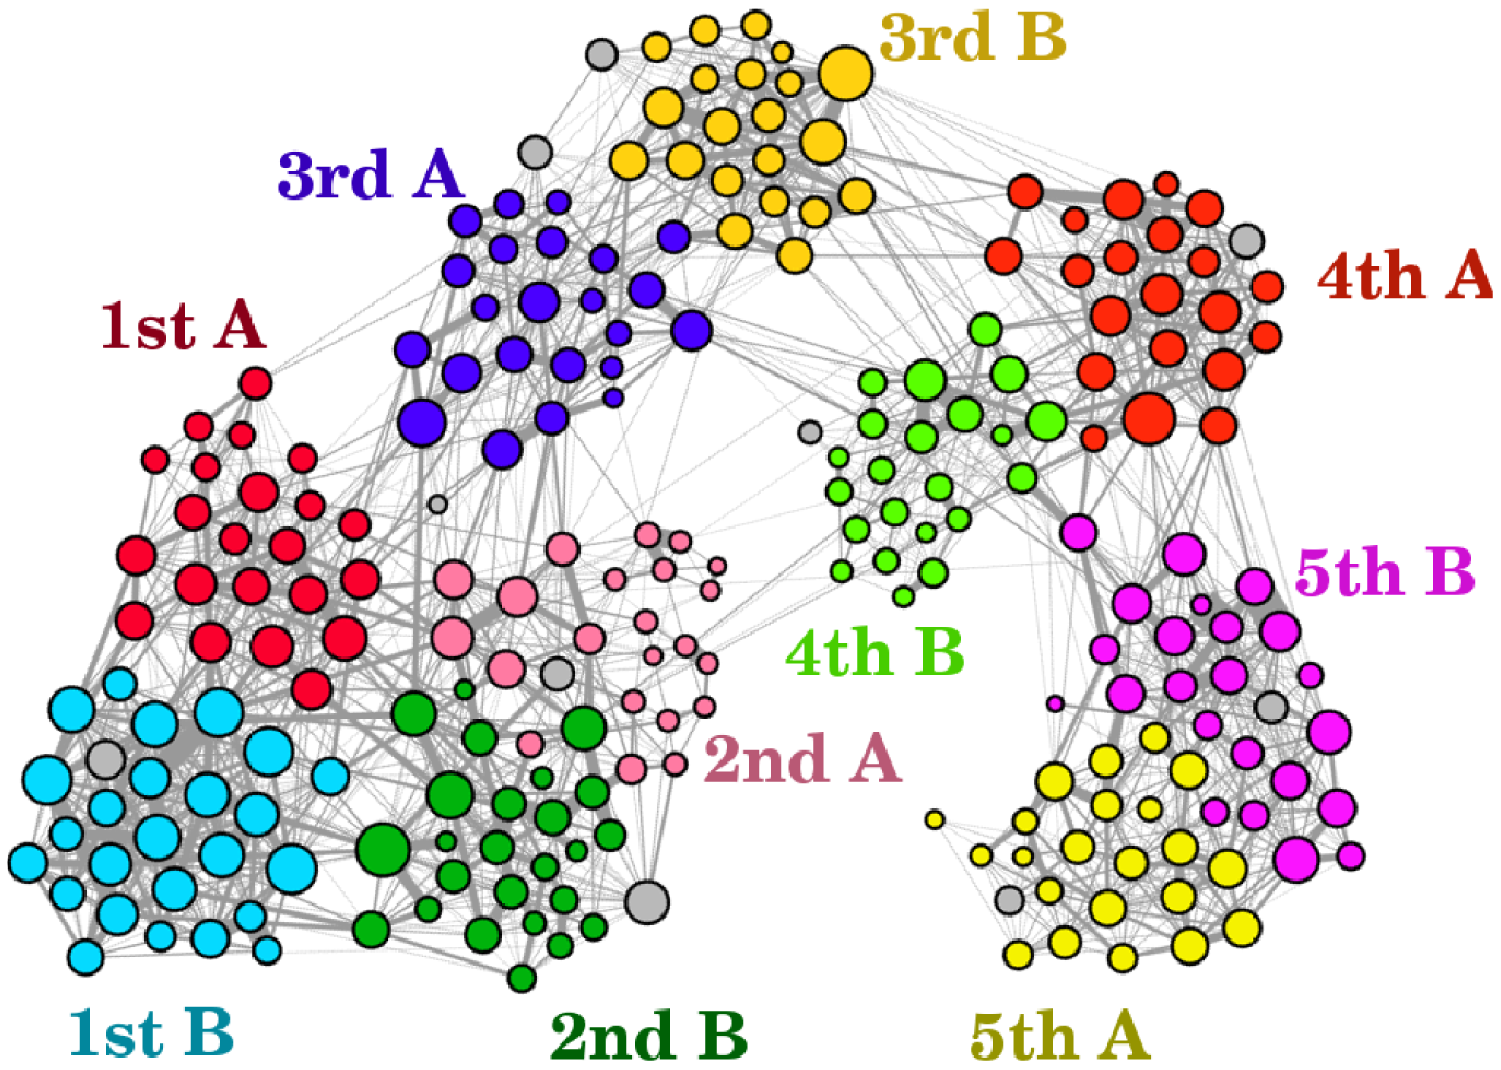
\includegraphics[width=0.7\linewidth]{img/Intro/ecole_primaire}
\caption{Graphe de contact des enfant d'une école primaire. L'épaisseur du lien représente la durée de communication entre deux élèves. La couleur représente la classe de chaque élèves. Les professeurs sont en gris.\protect\footnotemark}
\label{fig:ecole_primaire}
\end{figure}
\footnotetext{Image provenant de \url{http://journals.plos.org/plosone/article?id=10.1371/journal.pone.0023176}.}

Afin de capturer des partitions de n\oe uds, beaucoup de méthodes existent.
Il y a d'ailleurs régulièrement des état de l'art qui sont publiés~\cite{Fortunato2010,Plantie2013a, Malliaros2013a, Harenberg2014a}.
Afin d'aider le lecteur, nous détaillons ici quelques unes des méthodes les plus utilisées.

\subsubsection{Méthodes utilisant un modèle pour la comparaison}

Comme une communauté est souvent définie comme devant être très connectée, le problème est de trouver une fonction capable d'évaluer la connexité d'une communauté.
Pour ce faire, deux \emph{ingrédients} sont nécessaires.
Tout d'abord, il faut définir une métrique qui mesure la connexité, \emph{e.g.} le nombre de liens dans un groupe.
Puis, il est nécessaire de définir comment utiliser la métrique pour considérer qu'un groupe est très connecté.
Il est possible d'utiliser une métrique en la normalisant par ses bornes minimum et maximum.
Avec cette métrique normalisée entre $0$ et $1$, un groupe est considéré comme très connectés si son évaluation est supérieur à un certain seuil.
Cette approche n'est cependant pas adaptée pour la recherche de communauté car elle ne tiens pas compte de la structure du graphe\,\footnote{C'est plus approprié dans la recherche des groupes les plus denses~\cite{Balalau2015}.}.
Prenons l'exemple du graphe constitué d'une clique et du nombre de liens comme métrique.
Le nombre de lien d'un groupe est normalisé par le nombre minimum de liens, $0$, et par le nombre de maximum de liens qui est obtenu par une clique.
Dans ce graphe, tout groupe de n\oe uds est également une clique et par conséquent tout groupe de n\oe uds a un évaluation parfaite de $1$.
Chaque groupe serait donc une très bonne communauté selon cette évaluation.
Or, le graphe constitué d'une unique clique ne possède pas de structure communautaire contrairement au graphe dans la figure~\ref{fig:ecole_primaire}.
Il est donc nécessaire de trouver une autre approche.

Plutôt que de normaliser une métrique par ces valeurs minimum et maximum, il est intéressant de considérer l 'écart à une valeur moyenne.
L'idée est la suivante: si le graphe n'avait pas de structure communautaire qu'elle serait la valeur attendue de la métrique considérée?
Le problème est alors de définir des graphes qui n'ont pas de structures communautaires.
L'ensemble des graphes similaires définit alors un \emph{modèle nul}.
Détecter des communautés se traduit alors en trouver des groupes qui s'éloignent du modèle nul considéré où il n'existe pas de communauté.
Ce changement est astucieux car il est relativement aisé de définir des graphes n'ayant pas de structure.
Il suffit de créer des graphes complètement aléatoires~\cite{Erdos1959} où les liens du graphes sont tirés de manière uniforme.
Afin que les graphes aléatoires puissent être comparable au graphe initiale, des contraintes sont généralement ajoutées et donnent lieu à différent modèle nul.
Le premier modèle nul de graphe est celui de Erdös-Rényi~\cite{Erdos1959} où le nombre de liens et le nombre de n\oe uds des graphes aléatoires doivent être les mêmes que dans le graphe initial.
Un autre modèle très couramment utilisé est le modèle de configuration~\cite{Bender1978a}.
Dans ce modèle, la distribution des degrés est également fixe.
Le modèle est de configuration est souvent utilisé car il a été souvent observé que les graphes provenant de données réelles ont une distribution des degrés très éloignés d'une distribution uniforme.
C'est pourquoi l'ajout de la contrainte sur les degrés permet de considérer des graphes dans le modèle nul plus similaire au graphe initiale. 
Ils existent bien évidement d'autres modèles possibles considérant d'autres contraintes~\cite{Newman2009}.

\paragraph{Modularité}
La modularité~\cite{Newman2004} est une fonction qui associe a chaque partition de n\oe uds une valeur de qualité entre $-1$ et $1$.
Plus la valeur de modularité d'une partition est élevée, plus la partition est censée capturer une structure communautaire.
La modularité est définie de la manière suivante pour une partition $\mathcal{C}$:

\begin{equation}
Q(\mathcal{C}) = \dfrac{1}{2M}\sum_{i,j \in V} \left(A_{ij} - \dfrac{d_id_j}{2M}\right)\ \delta_{C(i)=C(j)} \ .
\end{equation}
Il s'agit pour deux n\oe uds d'une même communauté de comparer la présence ou absence d'un lien,$A_{ij}$, à la probabilité que ces des n\oe uds soient reliés dans le modèle de configuration, $\dfrac{d_id_j}{2M}$.
L'idée sous-jacente est que les n\oe uds d'une communauté devraient partager plus de liens qu'espéré dans le modèle de configuration.
De très nombreux travaux ont par la suite étudié les caractéristiques de la modularité et son optimisation.
Tout d'abords, il a été montré que l'optimisation de la modularité est un problème NB-Complet~\cite{Brandes2007}.
Il est donc nécessaire de recourir à des heuristiques afin de trouver rapidement une partition proche de l'optimum
Parmi l'ensemble des algorithmes existant, l'algorithme de Louvain~\cite{Blondel2008a} est un des plus rapide.
Il existe également des variantes de cet algorithme~\cite{Huang2015,Traag2015a}.
D'autres travaux se sont attachés à l'étude de la modularité.
Il a été montré que la modularité souffre du problème de \emph{résolution limite}~\cite{Fortunato2007,Lancichinetti2011} car le modèle de configuration présuppose une répartition uniforme des tailles des communautés.
Il a par ailleurs été montré que la modularité n'offre pas de maximum clair et que beaucoup de partitions différentes ont des évaluations proches~\cite{Good2010}.
Pour répondre à ces problèmes, il existe des variantes~\cite{Reichardt2006,Delvenne2010}.

\paragraph{Surprise}
La fonction Surprise~\cite{Aldecoa2011,Traag2015b} est une autre fonction de qualité qui se base quant a elle sur le modèle de Erdös-Rényi pour évaluer la surprise d'observer un groupe de n\oe uds relié par $l$ liens.

\paragraph{Stochastic Block Model}
Nous avons définis précédemment la notion de modèle nul permettant de se comparer à l'absence de communautés.
Il est également possible de modéliser une structure communautaire puis de vérifier \emph{a posteriori} si ce modèle pourrait être à l'origine du graphe observé.
Le problème de détection de communauté est alors un problème d'inférence qui est traité avec des outils statistiques tel que le \emph{stochastic block model} (SBM)~\cite{Holland1983a,Nowicki2001}.
L'idée derrière le SBM est la suivante: la probabilité que deux n\oe uds soient reliés dépend uniquement de leur groupe respectif.
Si le graphe a une structure communautaire, alors deux n\oe uds d'une même communauté devraient avoir une forte chance d'être connecté.
\`A l'inverse, deux n\oe uds de deux communauté différentes devraient avoir une probabilité assez faible d'être connecté.
Le SBM est défini par de nombreux paramètres: le nombre de groupe, l'assignation d'un groupe à chaque n\oe ud et les probabilités d'interactions entre les groupes.
Avec un jeu de paramètres donné, il est alors possible de calculer la vraisemblance que ce jeu de paramètre soit à l'origine du graphe.
Trouver une partition de n\oe uds dans ce contexte est alors équivalent à trouver le jeu de paramètre qui est le plus vraisemblablement à l'origine du graphe.

Dans le SBM, tout les n\oe uds sont considérés comme équivalents en particulier vis-a-vis du degré ce qui n'est pas le cas dans beaucoup de graphes provenant de données réelles.
C'est pourquoi une version tenant compte du degré des n\oe uds a été proposée: le Degree-correcte Stochastic Block Model (DBSM)~\cite{Karrer2011}.
Enfin d'après de récents travaux\cite{Newman2016}, il semblerait que le DSBM et l'optimisation de la modularité soient liés.

\subsubsection{Méthodes utilisant des marches aléatoires}
Il existe de nombreuses autres approches que celles utilisant un modèle nul ou un modèle générateur.
Notamment, il y a des méthodes utilisant les marches aléatoires \cite{Pons2005,Rosvall2008}.
Ces méthodes tirent partis du fait que si une communauté est densément connectée alors un marcheur aléatoire devrait y rester assez longtemps.
En particulier, la méthode Infomap~\cite{Rosvall2008} repose sur une idée très élégante; une partition de n\oe uds est une carte du graphe et, en ce sens, elle doit aider sa lecture.
Une carte est efficace si elle permet de mieux comprendre l'objet d'étude en réduisant sa complexité.
Dans une carte d'un pays, les départements découpent l'espace en zones compactes et la plupart du temps la majorité des routes se retrouvent à l'intérieur des départements.
Ainsi un voyageur se déplaçant aléatoirement sur les routes a peu de chance de sortir d'un département.
Pour décrire, \emph{a posteriori}, l'ensemble des routes prises par ce voyageur, il suffit alors de donner le département initiale puis la liste des routes empruntées.
Il n'est pas nécessaire de répéter le département à chaque fois si le voyageur n'en est pas sortit.
En ce sens, la découpe d'un pays en département permet de réduire la complexité du voyage.
Il s'agit donc d'un problème lié à la théorie de l'information et de sa compression.
De manière similaire, Rosval~\emph{et al.} utilise des marcheurs aléatoires se déplaçant sur les n\oe uds du graphe et les communautés forment des zones du graphe.
Si les communautés sont bien formées et que les marcheurs aléatoires restent bloqués à l'intérieur, alors la description de leur marche aléatoire sera courte.
La longueur de cette description devient alors la signature de la partition et plus la signature est courte, meilleur la partition est.

La méthode a également été étudiée pour voir si elle souffre de \emph{résolution limite} comme la modularité~\cite{Kawamoto2015}.
Il semble que cet effet existe également dans Infomap mais qu'il soit beaucoup moins prononcé.

\paragraph{Autres méthodes}
Il existe bien d'autres méthodes pour détecter des communautés en tant que partition de n\oe uds.
Il y a les méthodes spectrales~\cite{Donetti2004,Mitrovic2009} qui se base sur les vecteurs propres de la représentation d'un graphe sous la forme d'une matrice.
De manière moins formelle, les méthodes sont des algorithme de propagations de labels (LPA)~\cite{Raghavan2007a,Li2014c}.
Dans ces méthodes, chaque n\oe uds a initialement un label puis à chaque itération chaque n\oe ud prend comme label un des label de ses voisins.
En général, un n\oe ud prend comme label celui qui est le plus présent parmi ses voisins.
Au bout d'un certain nombre d'itération ou l'équilibre, il ne reste que beaucoup moins de labels qui représentent les communautés.


\resume{Il existe de très nombreuses méthodes pour la détection de communautés en tant que partition de n\oe uds. Ils semblent que les méthodes d'optimisation de \textbf{modularité}, la méthode \textbf{infomap} et  les \textbf{Stochastic Block Model} soient les plus utilisées dans la littérature.}

\subsection{Couverture de n\oe uds}
\label{subsec:cover}
Jusqu'à maintenant nous avons considérons les communautés comme des partition de n\oe uds.
Or, les partitions sont très restrictives et ne peuvent pas capturer toutes les situations possibles.
Reprenons l'exemple d'un graphe reflétant des interactions de personnes comme dans la section~\ref{sec:intro_communaute}.
Ils existent des communautés qui sont disjointes comme le travail et la famille mais bien souvent des personnes appartenant à plusieurs groupes, voire l'exemple dans la figure~\ref{fig:ex_overlap_communaute}.
Ainsi le groupe de personnes faisant du sport ensemble et le groupe des personnes travaillant ensemble peuvent ne pas être disjoint.
Si tel est le cas, alors il n'est plus possible de représenter des communautés avec une partition.
Il est nécessaire de manipuler une couverture de n\oe uds.
Ainsi dans l'exemple dans la figure~\ref{fig:ex_overlap_communaute}, les n\oe uds rouges devraient appartenir deux groupes au lieu d'un seul.

\begin{figure}
	\centering
	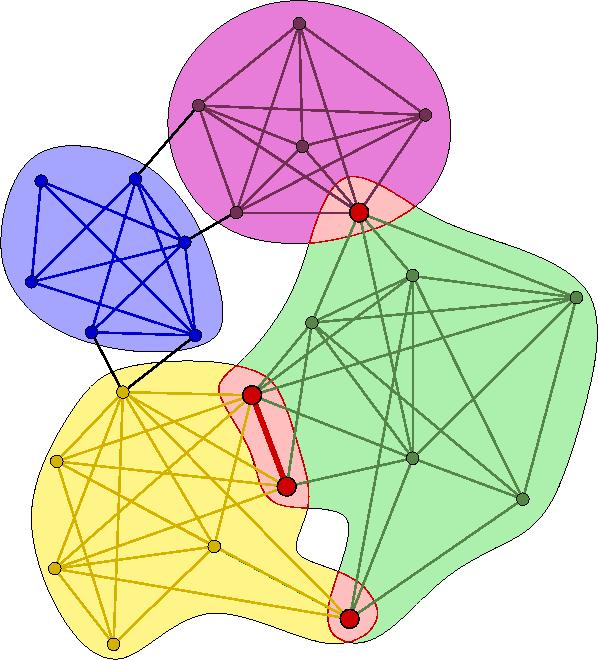
\includegraphics[width=0.31\linewidth]{img/Intro/Illustration_of_overlapping_communities.jpg}
	\caption{Exemple graphe avec une structure communautaire chevauchante représenté par les couleurs\,\protect\footnotemark.}
	\label{fig:ex_overlap_communaute}
\end{figure}
\footnotetext{Image provenant de \url{https://en.wikipedia.org/wiki/Clique_percolation_method}.}

Une fois encore, la littérature est très vaste dans ce domaine et nous ne ferons pas une liste exhaustive des méthodes existantes.
Pour une liste plus exhaustive, il existe de nombreux état-de-l'art dans le domaine~\cite{Danisch2012, Kanawati2014, Xie2013,Bandyopadhyay2015, Hric2014a}.

Une des premières méthodes de détection de couverture de n\oe uds est la \emph{Clique Percolation Method} (CPM)~\cite{Palla2005}.
L'algorithme CPM repose sur le principe de transitivité qui serait à l'origine des communautés: si $i$ et $j$ sont reliés par un lien alors le n\oe ud $k$ qui est déjà relié à $i$ a une forte chance d'être également connecté à $k$.
Il s'agit de la formalisation du proverbe "Les amis de mes amis sont mes amis".
Si ce principe est réellement à l'origine des communautés, alors elles doivent être composées de plusieurs cliques.
C'est pourquoi CPM cherche l'ensemble des cliques d'une taille $k$ donnée, en générale $k<10$ pour des raisons de coût de calcul, puis fusionne toutes les cliques qui partagent suffisamment de n\oe uds, en générale $k-1$. 
Comme cette méthode est relativement couteuse, Kumpula \emph{et al.}~\cite{Kumpula2008} ont repris le même mécanisme en optimisant le mode de calcul.

\subsubsection{Extension de méthodes existantes}

La majorité des méthodes existantes pour les partitions ont été adaptées pour manipuler les couvertures de n\oe uds.
Il existe plusieurs extensions de la modularité~\cite{Shen2009,Nicosia2009}.
Cependant ces extensions ne reposent plus sur un modèle nul car elles introduisent des termes de normalisations.
Par conséquent, ces extensions sont beaucoup moins utilisées que la modularité initiale.

\paragraph{Stochastic Block Model}
En revanche, le SBM s'adapte très bien aux couvertures de n\oe uds.
Une extension du SBM est le Mix-Membership Stochastic Block Model (MMSBM)\cite{Airoldi2008} qui permet à un n\oe uds d'avoir plusieurs groupes.
Dans~\cite{Gopalan2013a}, les auteurs utilisent la même méthodes mais en échantillonnant le graphe initiale afin de réduire le cout de calcul.
Il existe d'autres méthodes à base de modèle génératif~\cite{Ball2011,Yang2013}.
Ces méthodes se basent sur des graphe d'affiliation\cite{BreigerRonald1974}.
Un graphe d'affiliation est un graphe biparti entre les n\oe uds d'une part et les communautés de l'autre part.
Dans la méthode de Ball\emph{et al.}, ce graphe d'affiliation est pondéré et la pondération représente la propension d'un n\oe uds à créer des liens dans un groupe donné tant dis que dans Yang\emph{et al.} il s'agit du facteur d'appartenance du n\oe uds au groupe.
Une fois le graphe d'affiliation définit, il est nécessaire de savoir recréer la matrice d'adjacence et, en ce sens, ces méthodes se rapprochent des méthodes de factorisation non négative de matrices~\cite{Lee1999}.
Le but de la factorisation non-négative d'une matrice donnée est d'être capable de trouver deux matrices dont les entrées sont non-négatives tel que leur combinaison permettre de retrouver la matrice initiale.

Jusque récemment ce genre de technique généralisant le SBM ne pouvaient s'appliquer qu'à des graphes relativement petit.
il semble cependant que les méthodes récentes~\cite{Gopalan2013a, Yang2013} arrivent à traiter des graphes ayant énormément de liens, de l'ordre $10^{12}$ liens.



\paragraph{Propagation de label}
Des méthodes ont étendus la propagation de label aux couvertures de n\oe uds~\cite{Gregory2010,Xie2011}.
Le principal changement est qu'un n\oe ud ne stocke plus un unique label mais soit plusieurs labels soit des fréquences d'apparition de label.
Ainsi à la fin de l'algorithme, il suffit de choisir les labels les plus fréquents.
Cependant ce mécanisme de propagation change radicalement de l'idée initiale.
En effet, la diffusion d'un label n'est plus directement contrainte par la diffusion des autres labels.
Dans cette nouvelle configuration, il est possible qu'un label soit présent dans tout les n\oe uds.
De plus selon les auteurs de ces méthodes, des communautés non connexes peuvent apparaître ce qui nécessite l’ajout d’un mécanisme de post-processing.


\paragraph{Infomap}
Il s'agit surement de la méthode étant le moins "déformé" avec le SBM par l'adaptation aux partitions chevauchantes.
En effet, il suffit de relâcher la contrainte sur le fait qu'un n\oe ud n'appartienne qu'à un seul groupe.
Il est toujours possible de décrire un trajet par un nom de groupe puis une liste de n\oe uds visités dans le même groupe.
Ainsi, la notion de longueur de description est toujours valide même dans contexte.
Ce travail d'extension a été fait par Esquivel\emph{et al.}~\cite{Esquivel2011}.

\subsubsection{Méthodes utilisant des fonctions de qualité locales}
On a vu avec la modularité qu'il est assez difficile de définir une fonction de qualité évaluant une couverture de n\oe uds en fonctions des caractéristiques des groupes.
En revanche, les LPA tirent partis de l'information locale pour créer des groupes locales mais ne permettent pas leur évaluation.
L'idée est en quelque sorte mélanger ces deux aspects.
Il s'agit d'algorithmes qui initialement considèrent de très petites communautés puis essayent de les étendre itérativement en ajoutant des n\oe uds.
Afin de ne s'étendre un groupe indéfiniment comme cela peut être le cas avec les LPA, un ajout n'est fait que s'il améliore une fonction de qualité locale.
Ainsi dans ce type d'algorithme, il y a principalement deux critères important:
le choix des communautés initiales et le critère d'évaluation.
Dans la majorité des cas, chaque n\oe ud constitue une communauté. 
OSLOM\cite{Lancichinetti2011a} diffère de cette situation car OSLOM utilise comme point de départ une partition trouvée par l'algorithme de Louvain ou par infomap.

Les fonctions de qualité applicable sont très nombreuses et nous ne mentionneront que trois.
Tout d'abord, il est possible d'utiliser le degré relatif~\cite{Luo2008} d'un groupe comme critère.
Il s'agit du ratio entre le nombre de $l_{in}$ liens internes à un groupe de n\oe uds et du nombre de liens totale $l_{in}+l_{out}$:$ \dfrac{l_{in}}{l_{in}+l_{out}}$.
En effet, plus le degré relatif est élevé, plus le groupe est dense comparé à son voisinage et plus il a de forte chance d'être une bonne communauté. 
Cette formulation est assez proche de la conductance ou coupe normalisée\cite{Shi2000}:
\begin{equation}
\phi =\dfrac{l_{out}}{\min \left( 2(l_{in}+l_{out}),m-2(l_{in}-l_{out}) \right) }
\end{equation}

Ces deux notions se rapportent à la notion de densité vis-à-vis de leur voisinage.
Il également possible d'évaluer une communauté locale par rapport aux nombre de triangles présents de la communauté.
C'est ce que mesure la cohesion~\cite{Friggeri2011} pour un groupe de taille $k$: 
\begin{equation}
cohesion=\dfrac{\Delta_3}{ {k \choose 3} } \times \frac{\Delta_3}{\Delta_3+\Delta_2},
\end{equation}
où $\Delta_3$ est le nombre de triangle dont les 3 n\oe uds sont à l'intérieur du groupe et $\Delta_2$ est le nombre de triangle dont unqiement 2 n\oe uds sont à l'intérieur du groupe.

Différentes méthodes d'initialisation ainsi que fonctions de qualité sont déaillées dans l'article de Kanawati~\cite{Kanawati2014}.
Ces méthodes semblent très prometteuses car elles permettent de traiter efficacement de très grand graphe tout comme les LPA mais elles profitent des fonctions de qualité locales qui permettent d'une certaines manières d'évaluer le résultat obtenus.


\resume{
La littérature sur la détection de couverture de n\oe ud est encore très récente.
Il est donc délicat de commencer à tirer des conclusions.
Cependant, il semble que les extensions de la modularité ne soient pas réellement capable de trouver des couvertures de n\oe uds.
En plus d'infomap, c'est surtout les méthodes utilisant des modèles génératifs et celles utilisant des fonctions de qualité locales qui semblent les plus à même de capturer des couvertures de n\oe uds pertinentes.
Bien que souvent limité à de petit exemple, les modèles génératifs semblent maintenant capable de traiter des graphes de tailles importantes.
Les méthodes utilisant des fonctions de qualité locales sont quant à elle très rapide mais le choix de la fonction de qualité semble encore délicat.
}




%benchmark \cite{Lancichinetti2008,Lancichinetti2009b}

\section{Extension temporelle des graphes}
\label{sec:intro_extension_temporelle}

\cite{Hartmann2014}

application:
Diffusions \cite{Backlund2014, Gauvin2015} \cite{Karimi2013,Holme2014a,Horvath2014,Karsai2011,Kivela2012,Lambiotte2013,Lee2012,Perotti2014,Rocha2011,Scholtes2014,Scholtes2013}temporal network \cite{Jo2014} impact inter event time
Face-to-face interaction: \cite{Barrat2013,Asur2009}
Communauté TVG: \cite{Bassett2013,Bazzi2016}
Réseau de transport: \cite{Gallotti2015} multilayer
\subsection{snapshot}
multylayer \cite{Mucha2010,Kivela2014,Peixoto2015c},mathemical source\cite{DeDomenico2013}, survey générale (génération, percolation, diffusion) \cite{Boccaletti2014}

snap\cite{Asur2009,Bassett2013,Bazzi2014} + fenetre glissante
\cite{de2016detection,Rosvall2010} change point snap

effet time window \cite{Krings2012,Ribeiro2013} (ribeiro effet sur les random walk)

centralité de lien \cite{Takaguchi2012}

Communauté:
\cite{Sun2007} graphescope
\cite{Lin2008} facenet
\cite{DeDomenico2014} info map sur du multi layer
\cite{Chakrabarti2006,Chen2013} current + stabilité
Multylayer SBM\cite{Stanley2015} \cite{Corneli2016} SBM sur chaque tranche. proche\cite{Matias2015}
\cite{Gauvin2014}
\cite{Guo2014}
\cite{Hopcroft2004}
\cite{Kalavathi2015}
temps intrinsèque.
\cite{Albano2014}

Génération de: \cite{Granell2015, Karsai2014,Perra2012}

\subsection{TVG/Evolving}
\cite{Casteigts2011,Wehmuth2014}
\cite{Figueiredo2012} random walk.
\cite{Cazabet2010} conductance sur TVG
Suivi dans les snapshot de la force d'une communauté: \cite{Du2015}
\cite{Caceres2013} time scale on temporal networks 
\cite{Cordeiro2016} évolution modularité
\cite{Epasto2015} le plus dense à un instant
\cite{Sun2014}

\subsection{Flots de liens}
\cite{Holme2013a,Holme2015b,Holme2015} plein d'étude possible
Formalisation algébric \cite{Batagelj2015}.
bursty \cite{Karsai2012a,Karsai2011,Moinet2015,Stehle2010} inter event time \cite{Kivela2014a}, \cite{Malmgren2008,Malmgren2009} heavy tail, \cite{Rocha2013}

motif \cite{Kovanen2011a,Kovanen2013}.
Le formalisme de flot de liens est défini plus en profondeur dans le chapitre~\ref{chap:def_flot}.
randomwalk\cite{Starnini2012b}

\cite{Gaumont2016}
centralité \cite{Costa2015,Kim2012, Pfitzner2013a, Praprotnik2015,Scholtes2015,Takaguchi2016}
densité \cite{Viard2014a}

generateur \cite{Starnini2013,Vestergaard2014}